%%=============================================================================
%% Bijlage: Bewijsstukken
%%=============================================================================

\chapter{\IfLanguageName{dutch}{Technische bewijsstukken}{Technical evidence}}%
\label{app:bewijsstukken}

Deze bijlage bevat de technische bewijsstukken die gebruikt werden ter ondersteuning van de gecontroleerde validatie in Hoofdstuk~\ref{ch:validatie}. De bewijsstukken zijn gegroepeerd volgens de relevante hypothesen uit Hoofdstuk~\ref{ch:risicoanalyse}. Er worden geen wachtwoorden, tokens of andere gevoelige authenticatiegegevens opgenomen. Waar screenshots of fiches gevoelige gegevens bevatten, moeten deze vóór de finale indiening worden afgeschermd.

\section{\IfLanguageName{dutch}{Bewijsstukken bij H2: netwerksegmentatie en laterale bereikbaarheid}{Evidence for H2: network segmentation and lateral reachability}}%
\label{app:h2-netwerksegmentatie}

De testhost bevond zich tijdens de metingen in het beheer-/wifi-segment. Uit de netwerkconfiguratie blijkt dat de host het IP-adres \texttt{10.0.0.156} gebruikte, met \texttt{10.0.0.150} als default gateway, DHCP-server en DNS-server. Daarmee vormen de onderstaande metingen een validatie vanuit het perspectief van een intern toestel op het beheer-/wifi-netwerk.

\begin{verbatim}
    Wireless LAN adapter Wi-Fi:
    
    IPv4 Address. . . . . . . . . . . : 10.0.0.156(Preferred)
    Subnet Mask . . . . . . . . . . . : 255.255.255.0
    Default Gateway . . . . . . . . . : 10.0.0.150
    DHCP Server . . . . . . . . . . . : 10.0.0.150
    DNS Servers . . . . . . . . . . . : 10.0.0.150
    10.0.0.150
\end{verbatim}

Tabel~\ref{tab:bewijs-h2-connectiviteit} vat de belangrijkste connectiviteits- en routemetingen samen.

\begin{table}[H]
    \centering
    \small
    \caption[Connectiviteits- en routemetingen bij H2]{Connectiviteits- en routemetingen bij H2.}
    \label{tab:bewijs-h2-connectiviteit}
    \begin{tabular}{p{0.28\textwidth}p{0.28\textwidth}p{0.34\textwidth}}
        \hline
        \textbf{Test} & \textbf{Resultaat} & \textbf{Interpretatie} \\
        \hline
        \texttt{tracert 10.0.0.60} &
        Eén hop naar \texttt{10.0.0.60} &
        De NVR was rechtstreeks bereikbaar vanuit het beheer-/wifi-segment. \\
        \hline
        \texttt{tracert 192.168.0.212} &
        Route via \texttt{10.0.0.150} naar \texttt{192.168.0.212} &
        Er bestond een gerouteerd pad naar een component in de \texttt{192.168.0.0/24}-range. \\
        \hline
        \texttt{tracert 192.168.0.15} &
        Pad via \texttt{10.0.0.150}; daarna een melding \textit{Destination host unreachable} vanaf \texttt{192.168.0.212} &
        De individuele camera was niet rechtstreeks bereikbaar vanuit de testhost. \\
        \hline
        \texttt{ping 10.0.0.60} &
        Vier succesvolle replies &
        De NVR was bereikbaar. \\
        \hline
        \texttt{ping 192.168.0.212} &
        Vier succesvolle replies &
        De tussenliggende component was bereikbaar. \\
        \hline
        \texttt{ping 192.168.0.15} &
        \textit{Destination host unreachable} vanaf \texttt{192.168.0.212} &
        Rechtstreekse bereikbaarheid van de individuele camera werd niet aangetoond. \\
        \hline
    \end{tabular}
\end{table}

De traceroute naar de NVR toont dat \texttt{10.0.0.60} rechtstreeks bereikbaar was vanuit het segment van de testhost.

\begin{verbatim}
    PS C:\Users\emiel> tracert 10.0.0.60
    
    Tracing route to 10.0.0.60 over a maximum of 30 hops
    
    1     2 ms     2 ms     3 ms  10.0.0.60
    
    Trace complete.
\end{verbatim}

De traceroute naar \texttt{192.168.0.212} toont een pad via de router/default gateway \texttt{10.0.0.150}.

\begin{verbatim}
    PS C:\Users\emiel> tracert 192.168.0.212
    
    Tracing route to 192.168.0.212 over a maximum of 30 hops
    
    1     3 ms     2 ms     2 ms  10.0.0.150
    2     3 ms     2 ms     2 ms  192.168.0.212
    
    Trace complete.
\end{verbatim}

De traceroute naar een individueel camera-adres eindigde met een unreachable-melding. Dit betekent dat de ping of traceroute werd uitgevoerd vanaf de testhost, maar dat de foutmelding onderweg werd teruggestuurd door \texttt{192.168.0.212}.

\begin{verbatim}
    PS C:\Users\emiel> tracert 192.168.0.15
    
    Tracing route to 192.168.0.15 over a maximum of 30 hops
    
    1     2 ms     2 ms     2 ms  10.0.0.150
    2     3 ms     2 ms     2 ms  169.254.11.21
    3  192.168.0.212  reports: Destination host unreachable.
    
    Trace complete.
\end{verbatim}

Ook de ping naar \texttt{192.168.0.15} bevestigt dat de individuele camera niet rechtstreeks bereikbaar was vanuit het onderzochte segment.

\begin{verbatim}
    PS C:\Users\emiel> ping 192.168.0.15
    
    Pinging 192.168.0.15 with 32 bytes of data:
    Reply from 192.168.0.212: Destination host unreachable.
    Reply from 192.168.0.212: Destination host unreachable.
    Reply from 192.168.0.212: Destination host unreachable.
    Reply from 192.168.0.212: Destination host unreachable.
    
    Ping statistics for 192.168.0.15:
    Packets: Sent = 4, Received = 4, Lost = 0 (0% loss),
\end{verbatim}

\section{\IfLanguageName{dutch}{Bewijsstukken bij H3: actieve beheer- en streamingdiensten}{Evidence for H3: active management and streaming services}}%
\label{app:h3-diensten}

Voor H3 werd nagegaan welke relevante diensten vanuit de testhost bereikbaar waren. De testen werden uitgevoerd met \texttt{Test-NetConnection}. Tabel~\ref{tab:bewijs-h3-poorten} geeft een overzicht van de vastgestelde poortbereikbaarheid.

\begin{table}[H]
    \centering
    \small
    \caption[Poortbereikbaarheid bij H3]{Poortbereikbaarheid van relevante componenten bij H3.}
    \label{tab:bewijs-h3-poorten}
    \begin{tabular}{p{0.22\textwidth}p{0.15\textwidth}p{0.18\textwidth}p{0.35\textwidth}}
        \hline
        \textbf{Host} & \textbf{Poort} & \textbf{Resultaat} & \textbf{Interpretatie} \\
        \hline
        \texttt{10.0.0.150} & 80 & Succesvol & HTTP-beheerinterface of webdienst bereikbaar. \\
        \hline
        \texttt{10.0.0.150} & 443 & Succesvol & HTTPS-poort bereikbaar. \\
        \hline
        \texttt{192.168.0.212} & 80 & Succesvol & HTTP-beheerinterface of webdienst bereikbaar. \\
        \hline
        \texttt{192.168.0.212} & 443 & Succesvol & HTTPS-poort bereikbaar. \\
        \hline
        \texttt{10.0.0.60} & 8000 & Succesvol & NVR-gerelateerde dienst bereikbaar. \\
        \hline
        \texttt{10.0.0.60} & 8888 & Succesvol & NVR-gerelateerde beheer- of toegangspoort bereikbaar. \\
        \hline
        \texttt{10.0.0.60} & 554 & Niet succesvol & RTSP-poort was vanuit het onderzochte segment niet bereikbaar. \\
        \hline
    \end{tabular}
\end{table}

De onderstaande outputs tonen dat webpoorten op de router/default gateway en op de component \texttt{192.168.0.212} bereikbaar waren vanuit de testhost.

\begin{verbatim}
    PS C:\Users\emiel> Test-NetConnection 10.0.0.150 -Port 80
    
    ComputerName     : 10.0.0.150
    RemoteAddress    : 10.0.0.150
    RemotePort       : 80
    InterfaceAlias   : Wi-Fi
    SourceAddress    : 10.0.0.156
    TcpTestSucceeded : True
\end{verbatim}

\begin{verbatim}
    PS C:\Users\emiel> Test-NetConnection 10.0.0.150 -Port 443
    
    ComputerName     : 10.0.0.150
    RemoteAddress    : 10.0.0.150
    RemotePort       : 443
    InterfaceAlias   : Wi-Fi
    SourceAddress    : 10.0.0.156
    TcpTestSucceeded : True
\end{verbatim}

\begin{verbatim}
    PS C:\Users\emiel> Test-NetConnection 192.168.0.212 -Port 80
    
    ComputerName     : 192.168.0.212
    RemoteAddress    : 192.168.0.212
    RemotePort       : 80
    InterfaceAlias   : Wi-Fi
    SourceAddress    : 10.0.0.156
    TcpTestSucceeded : True
\end{verbatim}

\begin{verbatim}
    PS C:\Users\emiel> Test-NetConnection 192.168.0.212 -Port 443
    
    ComputerName     : 192.168.0.212
    RemoteAddress    : 192.168.0.212
    RemotePort       : 443
    InterfaceAlias   : Wi-Fi
    SourceAddress    : 10.0.0.156
    TcpTestSucceeded : True
\end{verbatim}

Voor de NVR op \texttt{10.0.0.60} waren poorten \texttt{8000} en \texttt{8888} bereikbaar. Poort \texttt{554}, typisch geassocieerd met RTSP, was vanuit het onderzochte segment niet bereikbaar.

\begin{verbatim}
    PS C:\Users\emiel> Test-NetConnection 10.0.0.60 -Port 8000
    
    ComputerName     : 10.0.0.60
    RemoteAddress    : 10.0.0.60
    RemotePort       : 8000
    InterfaceAlias   : Wi-Fi
    SourceAddress    : 10.0.0.156
    TcpTestSucceeded : True
\end{verbatim}

\begin{verbatim}
    PS C:\Users\emiel> Test-NetConnection 10.0.0.60 -Port 8888
    
    ComputerName     : 10.0.0.60
    RemoteAddress    : 10.0.0.60
    RemotePort       : 8888
    InterfaceAlias   : Wi-Fi
    SourceAddress    : 10.0.0.156
    TcpTestSucceeded : True
\end{verbatim}

\begin{verbatim}
    PS C:\Users\emiel> Test-NetConnection 10.0.0.60 -Port 554
    WARNING: TCP connect to (10.0.0.60 : 554) failed
    
    ComputerName           : 10.0.0.60
    RemoteAddress          : 10.0.0.60
    RemotePort             : 554
    InterfaceAlias         : Wi-Fi
    SourceAddress          : 10.0.0.156
    PingSucceeded          : True
    PingReplyDetails (RTT) : 2 ms
    TcpTestSucceeded       : False
\end{verbatim}

\section{\IfLanguageName{dutch}{Bewijsstukken bij H4: remote access en DNS-validatie}{Evidence for H4: remote access and DNS validation}}%
\label{app:h4-remote-dns}

De installatiefiche vermeldt historische configuratiegegevens voor externe toegang, waaronder een DynDNS-hostname en toegang via poort \texttt{8888}. De fiche wordt opgenomen als bewijsstuk, maar gevoelige gegevens zoals wachtwoorden moeten afgeschermd worden.

\begin{figure}[H]
    \centering
    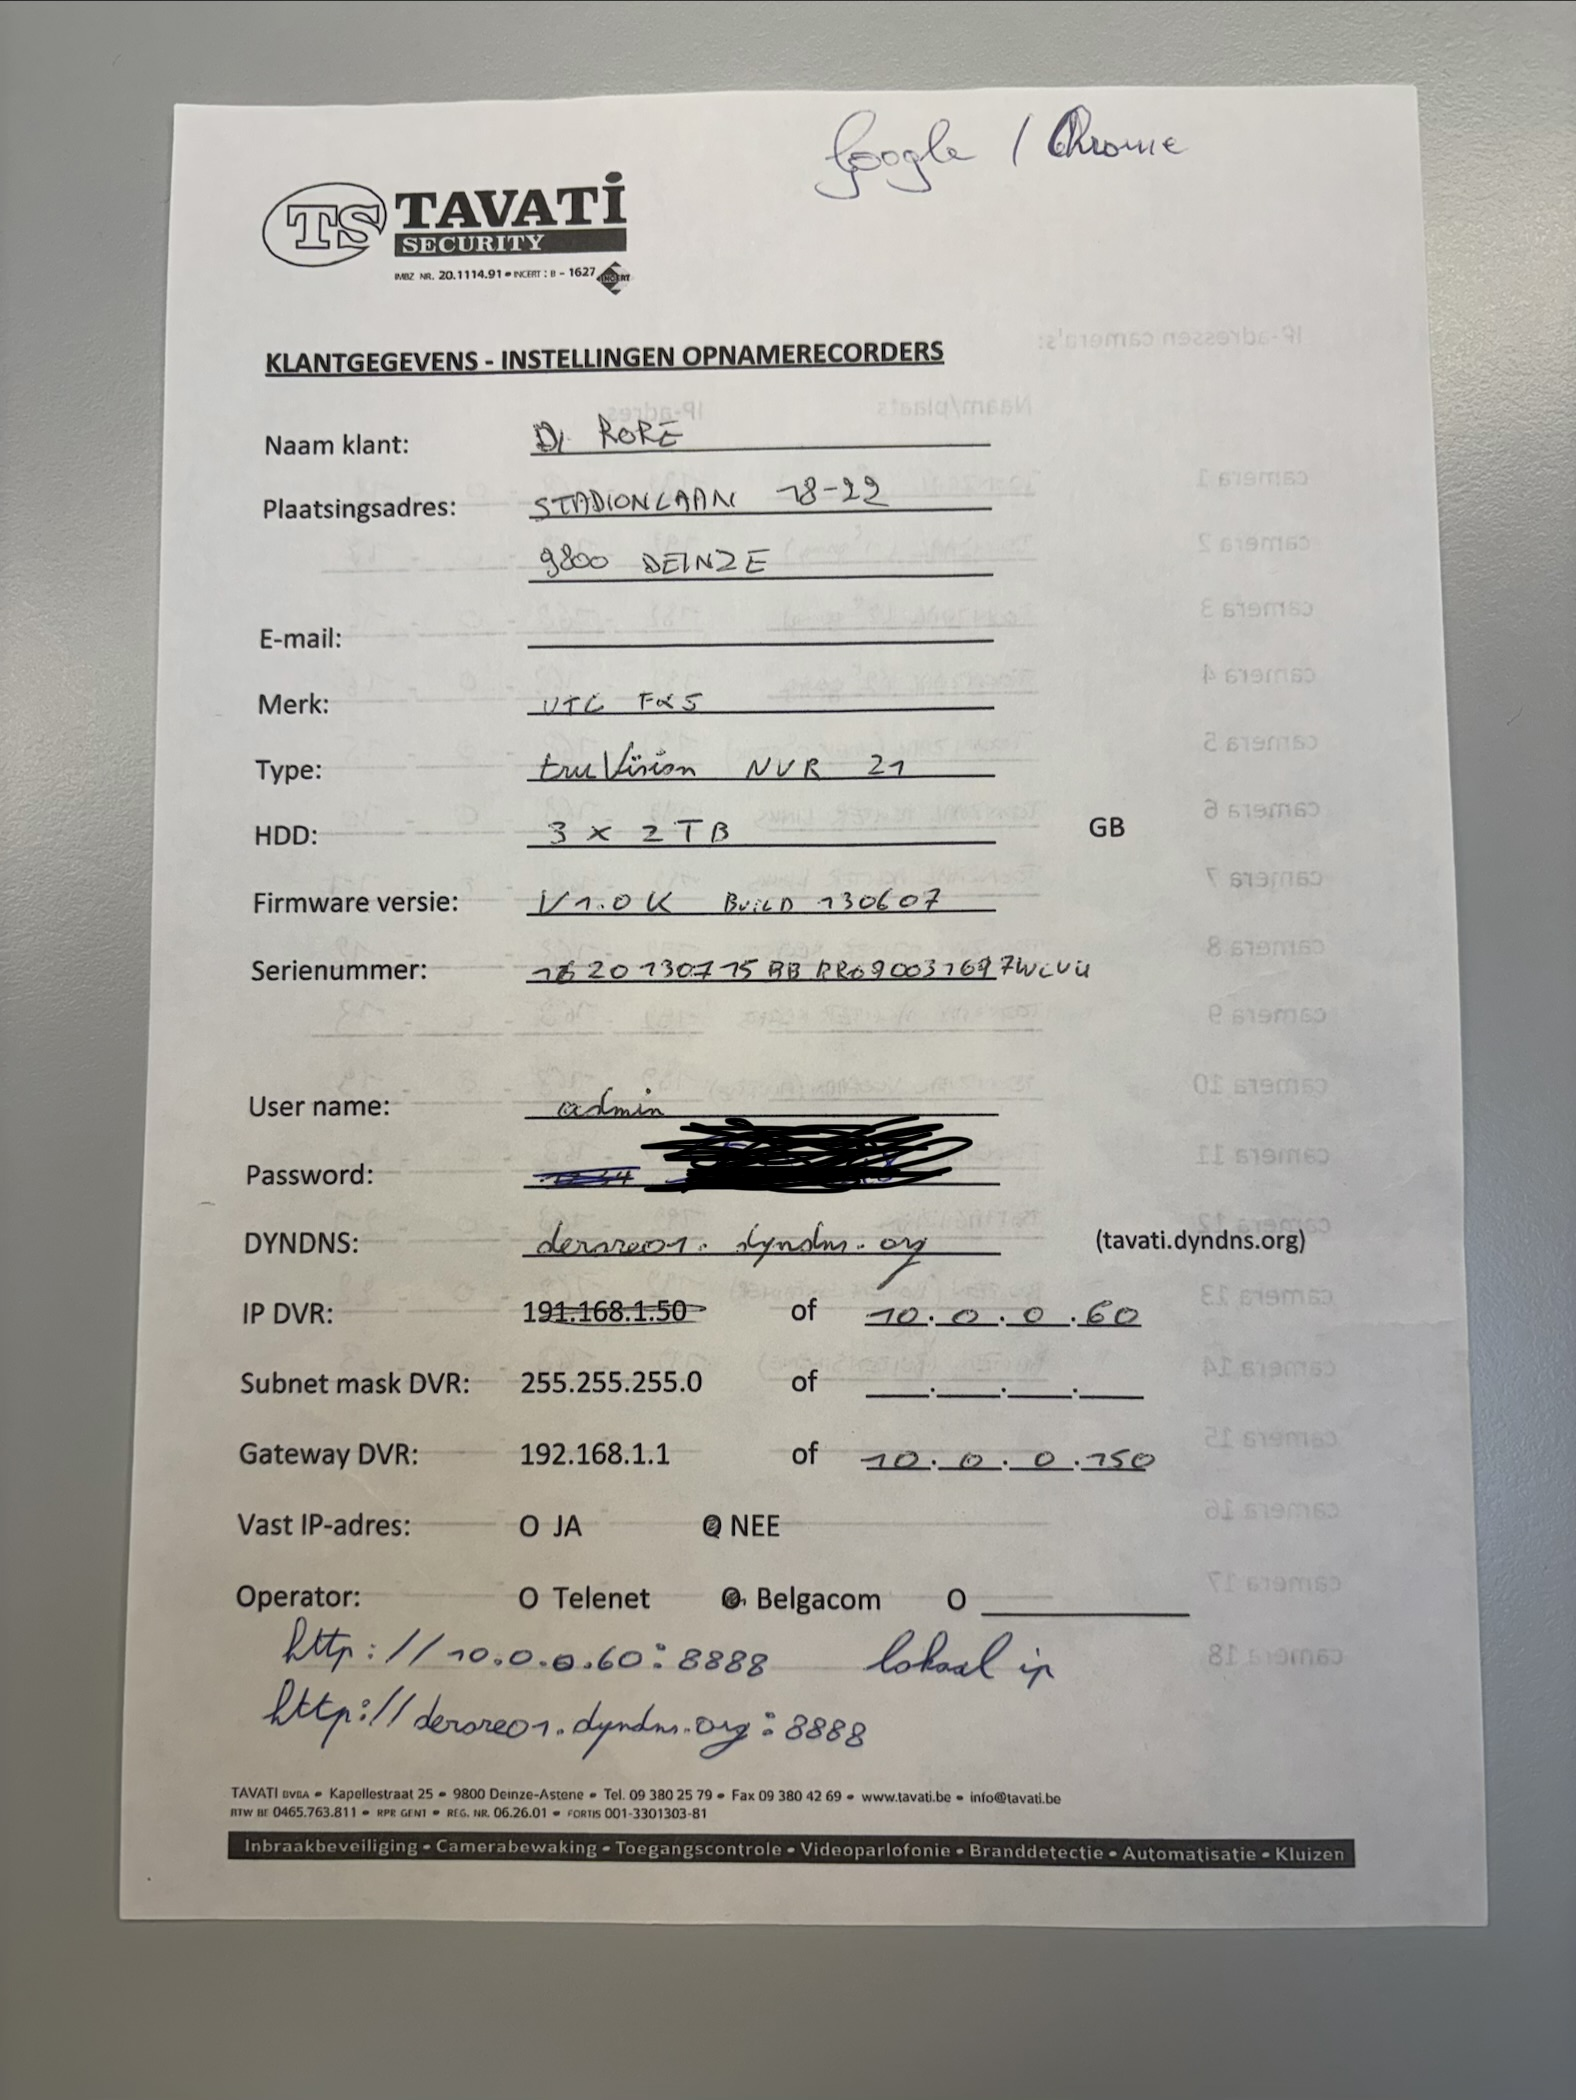
\includegraphics[width=.85\textwidth]{../Voorbereiding/Bewijsstukken/H1/tavati_installatiefiche}
    \caption[Installatiefiche met DynDNS-vermelding]{Installatiefiche van de camerarecorder met vermelding van configuratiegegevens zoals NVR-type, lokale toegang en historische DynDNS-instelling. Gevoelige gegevens werden afgeschermd.}
    \label{fig:bewijs-tavati-installatiefiche}
\end{figure}

De DNS-validatie toont dat de historische DynDNS-hostname nog resolveerde naar een publiek IP-adres.

\begin{verbatim}
    PS C:\Users\emiel> nslookup derore01.dyndns.org
    Server:  UnKnown
    Address:  10.0.0.150
    
    Non-authoritative answer:
    Name:    derore01.dyndns.org
    Address:  141.135.202.68
\end{verbatim}

De bijkomende TCP-connectiviteitstesten naar poorten \texttt{8000} en \texttt{8888} bevestigden echter geen externe bereikbaarheid op deze poorten.

\begin{verbatim}
    PS C:\Users\emiel> Test-NetConnection derore01.dyndns.org -Port 8000
    WARNING: TCP connect to (141.135.202.68 : 8000) failed
    WARNING: Ping to 141.135.202.68 failed with status: TimedOut
    
    ComputerName           : derore01.dyndns.org
    RemoteAddress          : 141.135.202.68
    RemotePort             : 8000
    InterfaceAlias         : Wi-Fi
    SourceAddress          : 10.0.0.156
    PingSucceeded          : False
    PingReplyDetails (RTT) : 0 ms
    TcpTestSucceeded       : False
\end{verbatim}

\begin{verbatim}
    PS C:\Users\emiel> Test-NetConnection derore01.dyndns.org -Port 8888
    WARNING: TCP connect to (141.135.202.68 : 8888) failed
    WARNING: Ping to 141.135.202.68 failed with status: TimedOut
    
    ComputerName           : derore01.dyndns.org
    RemoteAddress          : 141.135.202.68
    RemotePort             : 8888
    InterfaceAlias         : Wi-Fi
    SourceAddress          : 10.0.0.156
    PingSucceeded          : False
    PingReplyDetails (RTT) : 0 ms
    TcpTestSucceeded       : False
\end{verbatim}

Deze resultaten tonen aan dat de DynDNS-hostname nog DNS-resolutie had, maar dat externe TCP-bereikbaarheid op de onderzochte poorten niet werd bevestigd.

\section{\IfLanguageName{dutch}{Bewijsstukken bij H5: logging en detecteerbaarheid}{Evidence for H5: logging and detectability}}%
\label{app:h5-logging}

Het bewijsstuk rond logging en controlegeschiedenis ondersteunt de beoordeling van H5. Dit bewijsstuk toont dat de beheeromgeving logcategorieën ondersteunt en minstens succesvolle aanmeldingen registreert. De operationele opvolging van deze logs wordt besproken in Hoofdstuk~\ref{ch:validatie}.


 \begin{figure}[H]
         \centering
         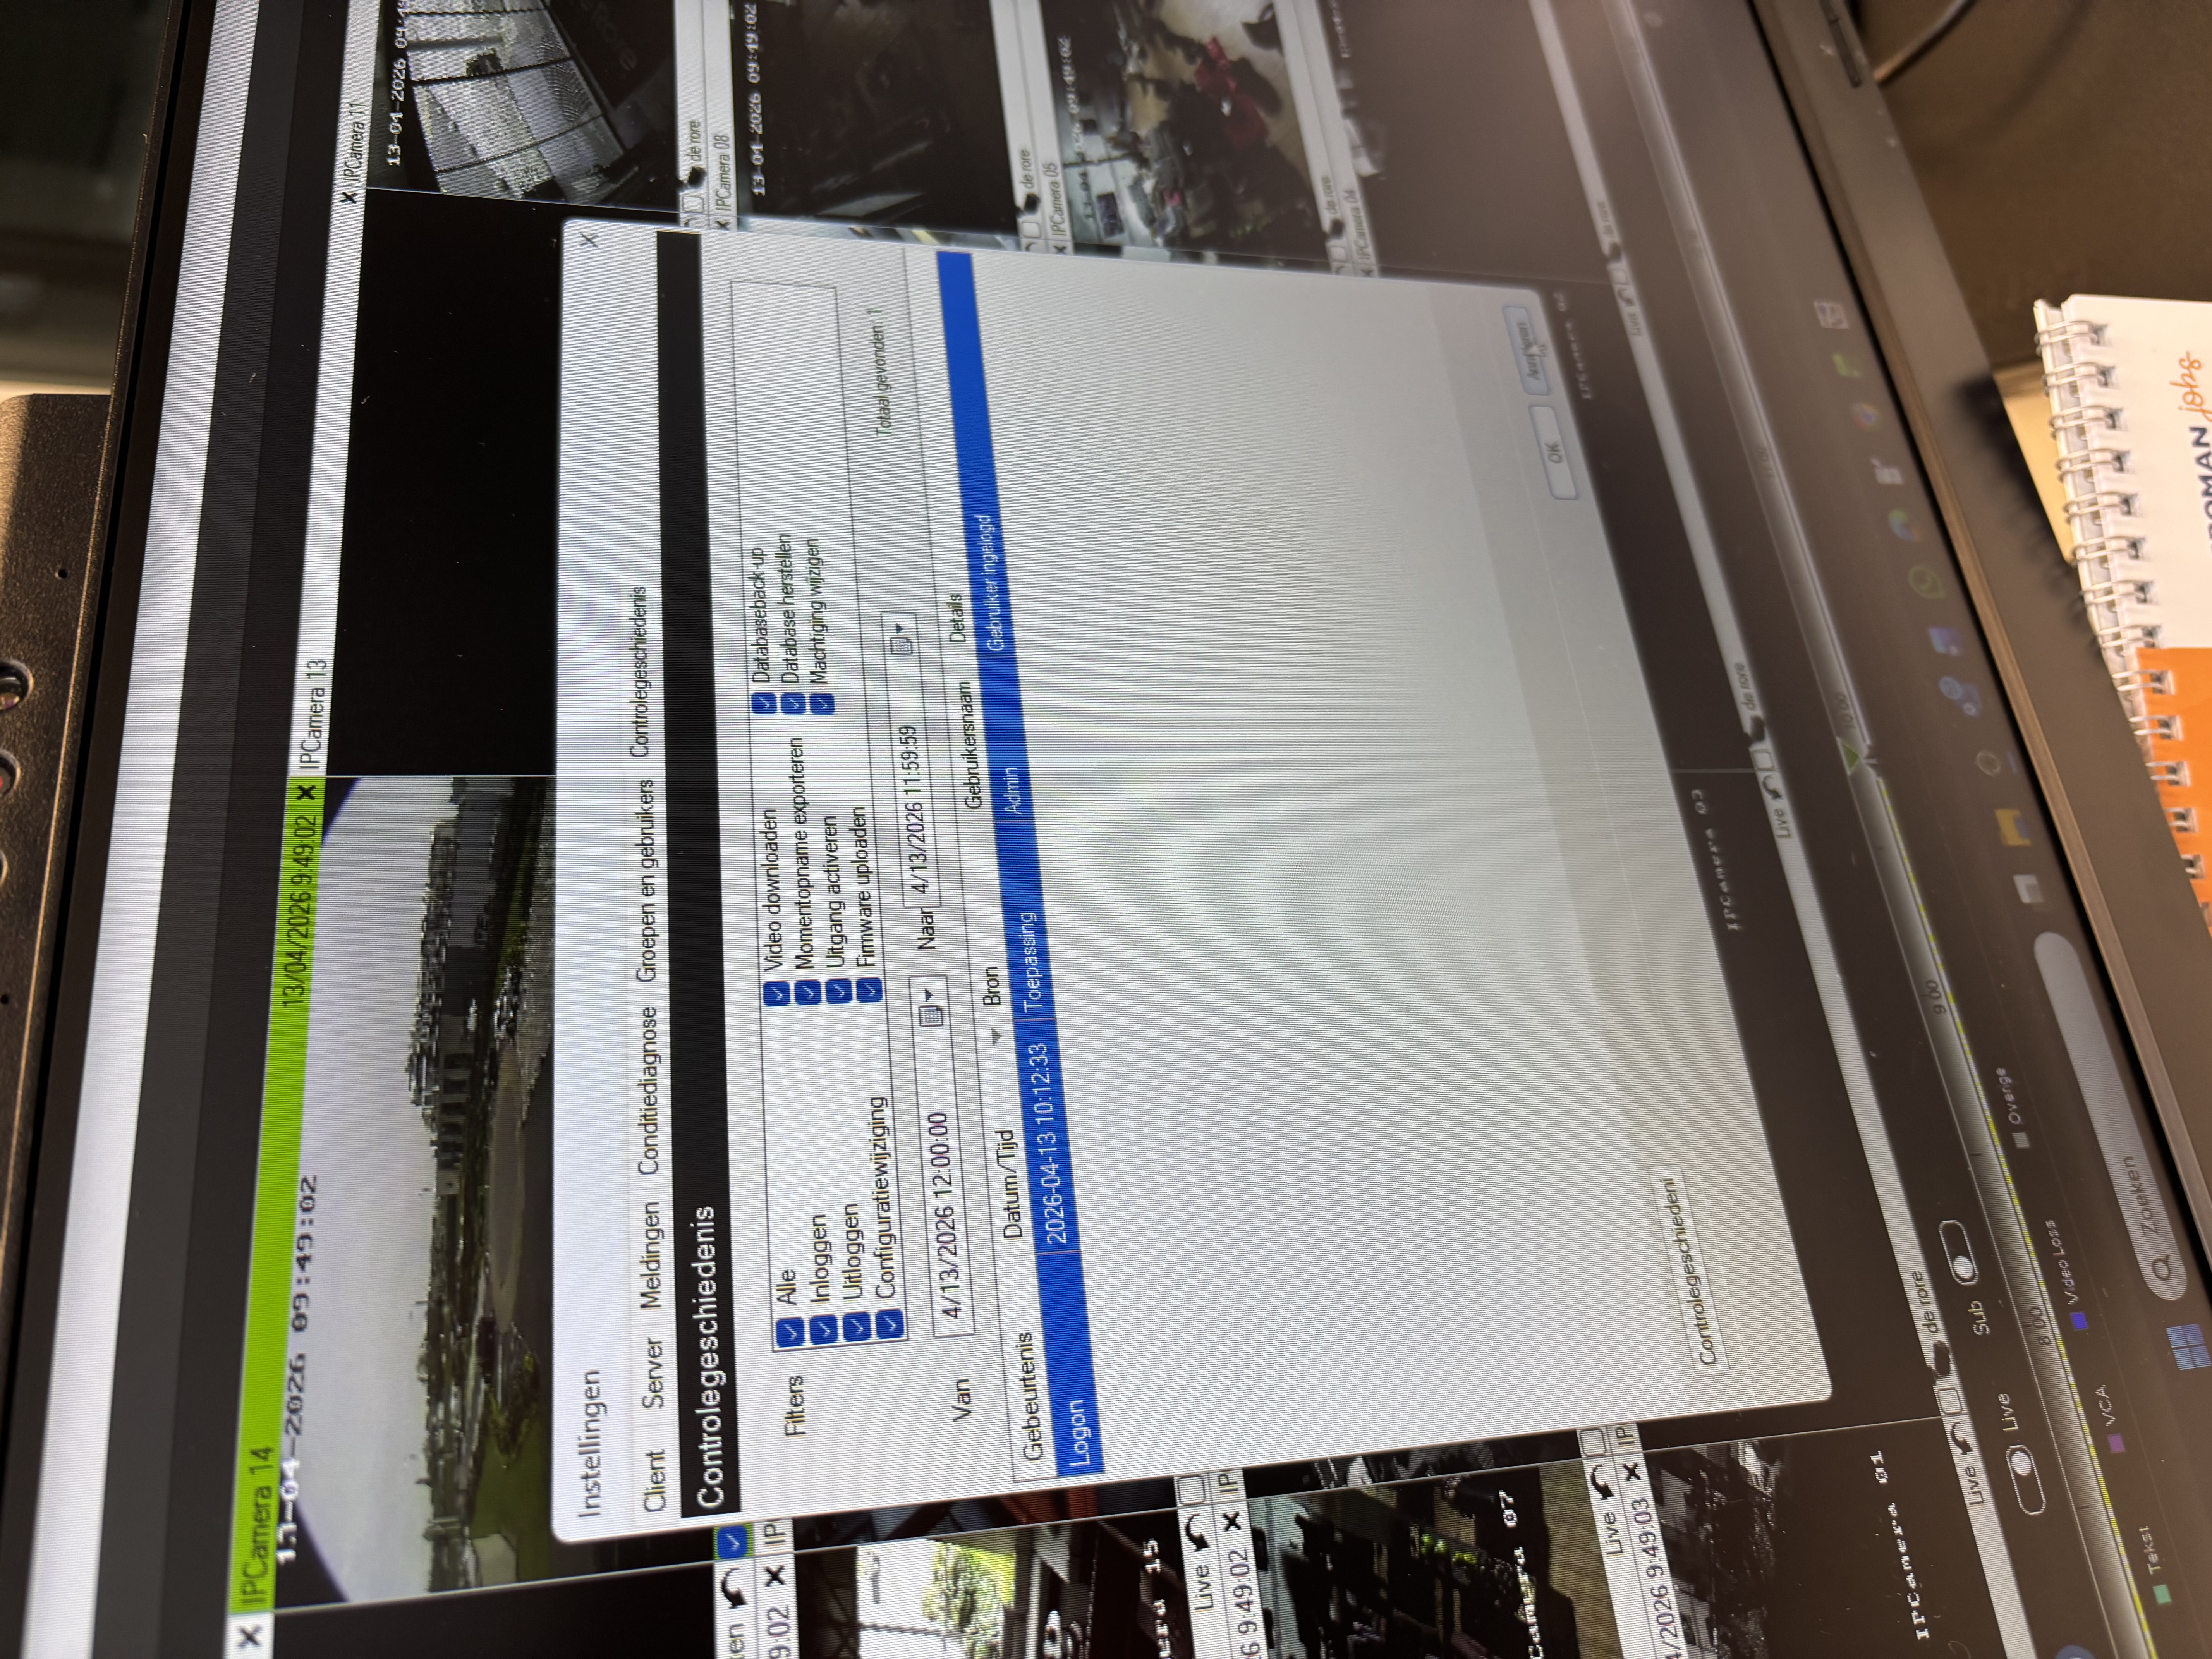
\includegraphics[angle=-90,width=.85\textwidth]{../Voorbereiding/Bewijsstukken/H1/logging_controlehistoriek}
         \caption[Controlehistoriek in TruVision Navigator]{Voorbeeld van de controlehistoriek in TruVision Navigator, met beschikbare logcategorieën en een geregistreerde succesvolle aanmelding.}
         \label{fig:logging-controlehistoriek}
     \end{figure}

